\usetikzlibrary{calc}


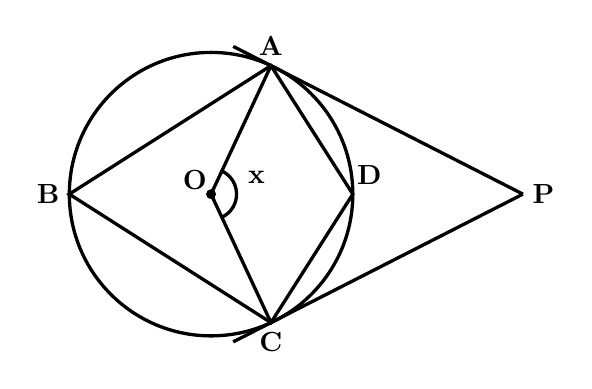
\begin{tikzpicture}[scale=1.8]
    % Define the circle radius
    \def\r{1}
    
    \coordinate (O) at (0,0);
    
    % Draw circle
    \draw[very thick] (O) circle (\r);
    
    % Define points on the circle for quadrilateral ABCD
    \coordinate (A) at (65:\r);
    \coordinate (B) at (180:\r);
    \coordinate (C) at (295:\r);
    \coordinate (D) at (0:\r);
    \coordinate (O) at (0,0);
    
    % External point P
    \coordinate (P) at (2.2,0);
    
    % Draw quadrilateral ABCD
    \draw[very thick] (A) -- (B) -- (C) -- (D) -- cycle;
    
    % Draw tangent lines PA and PC (extended beyond A and C)
    \draw[very thick] ($(A)!-0.15!(P)$) -- (P);
    \draw[very thick] ($(C)!-0.15!(P)$) -- (P);
    \draw[very thick] (O) -- (A);
    \draw[very thick] (O) -- (C);
    
    % Center point O with dot
    \fill (0,0) circle (1pt);
    
    % Draw small arc for angle x at O (from C at 295 degrees to A at 65 degrees, going clockwise through 0)
    \draw[very thick] (295:0.18) arc (295:360:0.18);
    \draw[very thick] (0:0.18) arc (0:65:0.18);
    
    % Labels with bold font
    \node[above, font=\bfseries] at (A) {A};
    \node[left, font=\bfseries] at (B) {B};
    \node[below, font=\bfseries] at (C) {C};
    \node[above right, font=\bfseries, xshift=-2pt] at (D) {D};
    \node[right, font=\bfseries] at (P) {P};
    \node[above left, font=\bfseries, xshift=2pt, yshift=-2pt] at (0,0) {O};
    \node[font=\bfseries] at (0.32,0.12) {x};
\end{tikzpicture}